\section{Case description} \label{ch:case description}

In this project, we are going to focus on the Universal Robot, UR5 which is an industrial manipulator.\\
The UR5 is going to assist in the balancing and leak test of a L40 rotor see \ref{fig:rotor} that is being produced at Grundfos. The L40 rotor is arriving at the work-cell via a conveyor belt. The rotor has to go through a balancing machine, where the rotor is placed in a drawer, after that it has to go through a visual inspection, before it has to be leak tested.\\
The leak testing machine can test two rotors per load, when the leak test is done, the machine will give a signal if the rotor has passed the test or not. If the rotor passes, it will be placed in an engraving machine that prints the ID of the rotor, after that it will be placed on a pallet, when it is full it will send a signal to a Grundfos employee to replace the pallet.\\ 
In between the leak machine and the engraving station we can utilize a table as a buffer which has 100 drilled holes for the rotor to be temporarily stored, furthermore the rotor has to has to go through this cycle in 26 seconds or less.\\
    

\begin{figure}
    \centering
    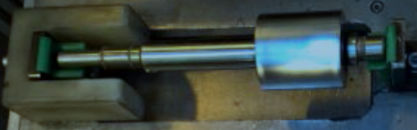
\includegraphics[width=9cm]{InitialProblemstatement/Case/rotorlille.PNG}
    \caption{The L40 rotor \cite{Case}}
    \label{fig:rotor}
\end{figure}



